
This chapter collects the full CFT schematics, in their latest
revision, including all peripherals. Please note that many schematics
are in various stages of incompleteness.

The state of each sheet of the schematics, including other details can
be found according to the key on the first sheet:

\begin{figure}[h!]
  \centering
  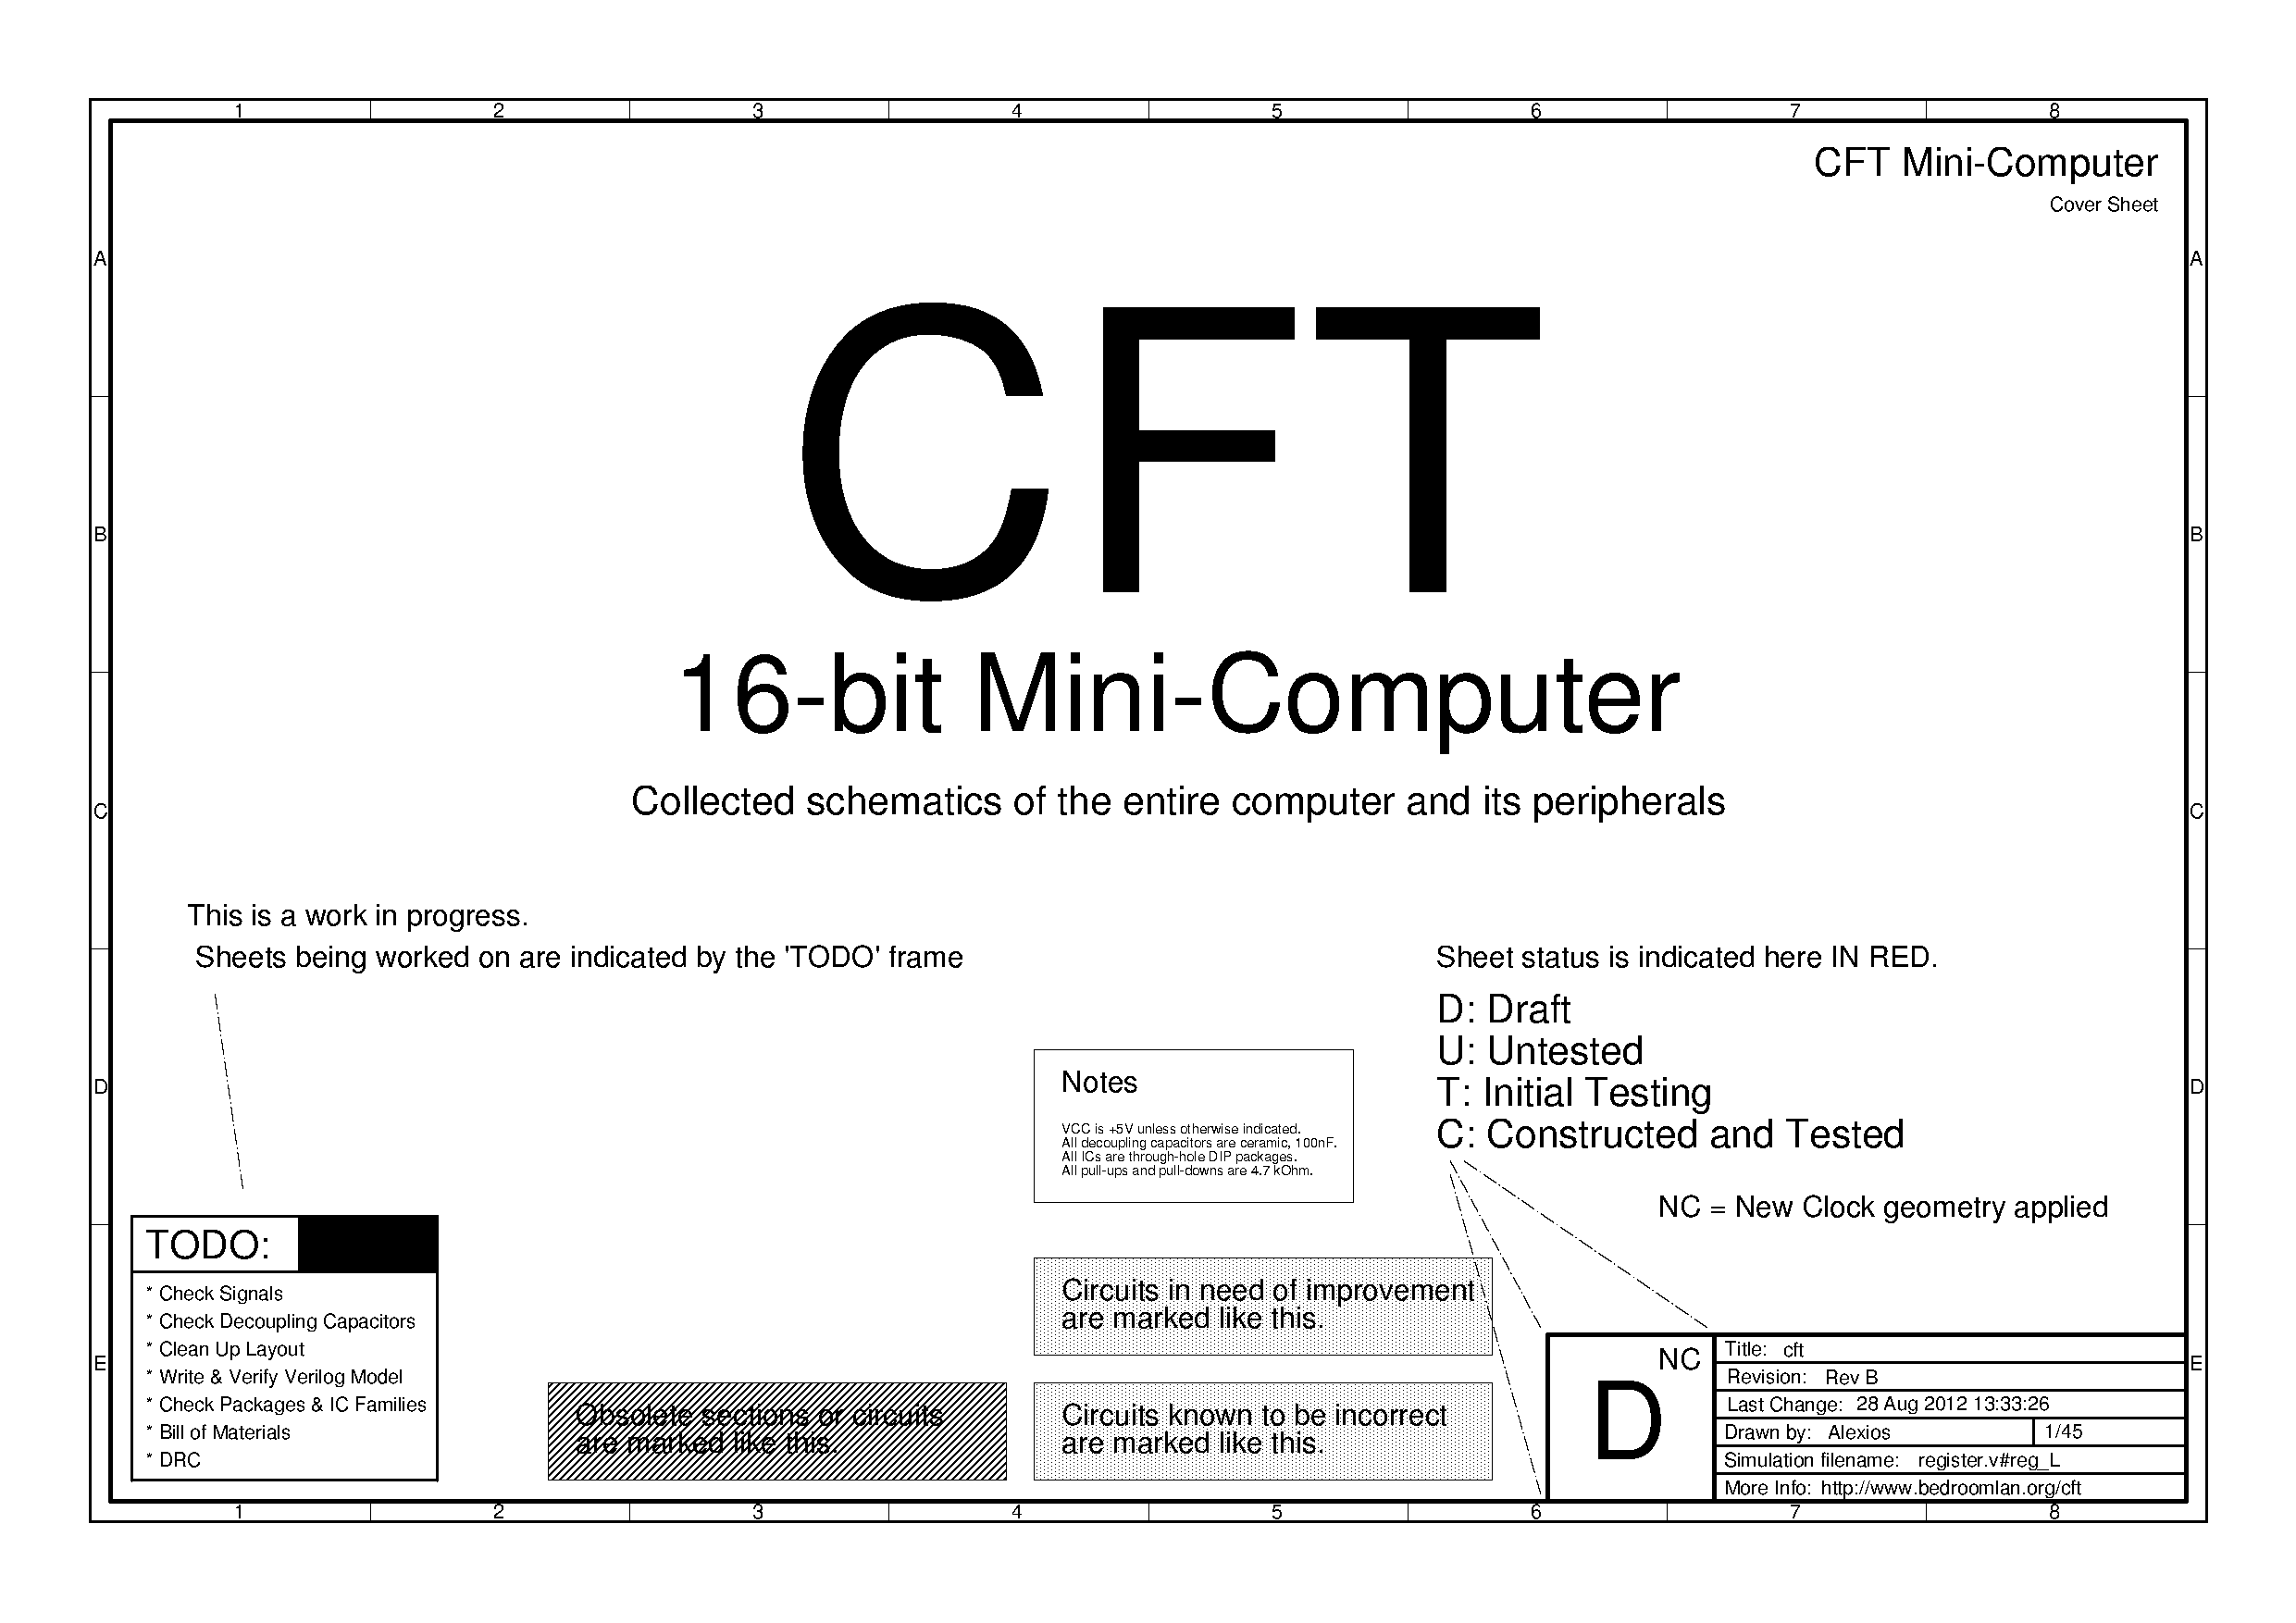
\includegraphics[width=\columnwidth]{figs/schematic-legend.pdf}
  \caption{\label{fig:schematic-legend}Schematic legend, explaining
    various markings and notation.}
\end{figure}

\newpage

\phantomsection\stepcounter{section}%
\addcontentsline{toc}{section}{\protect\numberline{\thesection} Processor Board A Schematics}

%% %\includesch{1}{Schematic cover page}{sch2:cover}
%% \includesch{2}{Clock Generation and control}{sch2:clock}
%% \includesch{3}{Reset Handling and Sequencing}{sch2:reset}
%% \includesch{4}{Microcode Sequencer}{sch2:useq}
%% \includesch{5}{Microcode Sequencer Signal Hold}{sch2:useq-hold}
%% \includesch{6}{Microcode Sequencer Front Panel Buffers}{sch2:useq-fp}
%% \includesch{7}{Read and Write Unit Decoding}{sch2:unit-decoders}
%% \includesch{8}{Skip and Branch Logic}{sch2:sbu}
%% \includesch{9}{Address Generation Logic}{sch2:agl}
%% \includesch{10}{Instruction Register}{sch2:ir}
%% \includesch{11}{Interrupt State Machine}{sch2:intsm}
%% \includesch{12}{Data Bus Driver and Bus Termination}{sch2:databus}

\phantomsection\stepcounter{section}%
\addcontentsline{toc}{section}{\protect\numberline{\thesection} Processor Board B Schematics}

%% \includesch{13}{Address Register, Address Bus Drivers \& Termination, Autoindex Logic and Device Decoder}{sch2:ar}
%% \includesch{14}{Program Counter}{sch2:pc}
%% \includesch{15}{Data Register}{sch2:dr}
%% \includesch{16}{Accumulator, Zero Flag and Negative Flag}{sch2:ac}

\phantomsection\stepcounter{section}%
\addcontentsline{toc}{section}{\protect\numberline{\thesection} Processor Board C Schematics}

%% \includesch{17}{Link Register}{sch2:l}
%% \includesch{18}{Arithmetic/Logic Unit: Decoders and Buffers}{sch2:aludecoder}
%% \includesch{19}{ALU Binary Operators}{sch2:alub}
%% \includesch{20}{ALU Unary Operators and Constant Store}{sch2:aluu}
%% \includesch{21}{8 kW Bank Switching Memory Controller}{sch2:mbu}

\phantomsection\stepcounter{section}%
\addcontentsline{toc}{section}{\protect\numberline{\thesection} Peripheral Schematics}

\includesch{22}{Interrupt Controller}{sch2:intc}
\includesch{23}{Control Bus Connectors}{sch2:cbus}
%%%\includesch{24}{Memory (RAM and ROM)}{sch2:memory}
\includesch{25}{RS-232 and TTL Serial Ports}{sch2:tty}
\includesch{26}{IDE Bus Interface}{sch2:ide}
\includesch{27}{Clock, Timers and NVRAM}{sch2:rtc}
\includesch{28}{Ethernet Interface}{sch2:eth}
\includesch{29}{PS/2 Keyboard Controller}{sch2:kbd}
\includesch{30}{Audio Device, bus interface and SpeakJet™}{sch2:sjs}
\includesch{31}{Audio Device, AY-3-8910 PSG}{sch2:psg}
%%%\includesch{42}{Debugging Board}{sch2:deb}

\phantomsection\stepcounter{section}%
\addcontentsline{toc}{section}{\protect\numberline{\thesection} Front Panel Schematics}

\includesch{32}{Front Panel: LEDs}{sch2:fp-leds}
\includesch{33}{Front Panel: Switch Register and Switches}{sch2:fp-switches}
%\includesch{34}{Front Panel: Switch Register and Switches}{sch2:fp-switches2}
\includesch{35}{Front Panel: Step switch auto-repeat}{sch2:fp-step-autorepeat}
%\includesch{36}{Front Panel: Switch Register and Switches}{sch2:fp-switches3}
%\includesch{37}{Front Panel: LEDs}{sch2:fp-leds2a}
\includesch{38}{Front Panel: Multi-Function Display Buffers}{sch2:fp-mfd}
\includesch{39}{Front Panel: Interrupt LED}{sch2:fp-irq-led-delay}
\includesch{40}{Front Panel: Connectors}{sch2:fp-con}
\includesch{41}{Front Panel: System Device}{sch2:pfp}
